\documentclass{beamer}
\usetheme{Szeged}
\usecolortheme{beaver}

\usepackage{minted}
\usemintedstyle{pastie}

\usepackage{graphicx}
\usepackage{hyperref}
\hypersetup{
    colorlinks=true,
    linkcolor=blue,
    filecolor=magenta,      
    urlcolor=cyan,
}

\title{Discussion 03}
\subtitle{Pattern Matching}
\author{Kenneth Fang (kwf37), Newton Ni (cn279)}
\date{Feb. 3, 2019}

\begin{document}

    \begin{frame}
        \titlepage{}
    \end{frame}
    
    \begin{frame}{Agenda}
    \begin{enumerate}
        \item Review concept of pattern matching
        
        \item Explore pattern matching with three different data structures:
            \begin{itemize}
                \item Lists v1::v2:: ... ::vn::[]
                \item Records \{label1=v1, label2=v2, ..., labeln = vn\}
                \item Tuples (v1,v2,...,vn)
            \end{itemize}
        
        \item Recitation 4
    \end{enumerate}
    \end{frame}
    
    \begin{frame}{What is Pattern Matching?}
    \pause
    \begin{itemize}
        \item How do we access data in arrays in an object-oriented language? \pause
        \item How do we access data in objects in an object-oriented language? \pause
        \item What if we extracted data by leveraging the \textit{structure} of the data? \pause
        \item When pattern matching, we can ensure that our data accesses are exhaustive and that every branch in the pattern match is being used
    \end{itemize}
    \end{frame}
    
    \begin{frame}{Lists}
        Lists in OCaml are
        \begin{itemize}
            \item Singly-linked lists
            \item Immutable
            \item ``First-class" data structures
        \end{itemize}
    \end{frame}
    
    \begin{frame}[fragile]{Lists}
    Lists are defined to be either 
    \begin{itemize}
        \item Nil \mintinline{ocaml}{[]}
        \item Cons \mintinline{ocaml}{h::t}
    \end{itemize} \pause
    
    Lists can be constructed using the following syntax:
    \begin{itemize}
        \item \mintinline{ocaml}{[]}
        \item \mintinline{ocaml}{e1::e2::e3::[]}
        \item \mintinline{ocaml}{[e1;e2;e3]} (syntactic sugar for above syntax)
    \end{itemize}
    Lists in OCaml are
    \end{frame}
    
    
    \begin{frame}{List Static Semantics}
    \begin{itemize}
        \item The empty list Nil has type \mintinline{ocaml}{'a list} \pause
        
        \item The list \mintinline{ocaml}{e1::[]} has type \mintinline{ocaml}{t list} if \mintinline{ocaml}{e1 : t} \pause
        
        \item All elements in a list must have the same type \pause
        
        \item For the cons operator \mintinline{ocaml}{h::t}, if \mintinline{ocaml}{h:typ}, then it must be true that \mintinline{ocaml}{t:typ list} \pause
        
        \item What is the type of the cons operator (::)?
    \end{itemize}
    \end{frame}
    
    \begin{frame}[fragile]{List Pattern Matching}
        Typically a list can be broken down as follows:
        \noindent\begin{minted}{ocaml}
            match lst with
            | [] -> (*Do something when list is empty*)
            | h::t -> (*Do something with head or tail*)
        \end{minted}
    \end{frame}
    
    \begin{frame}[fragile]{List Length}
    \mint{ocaml}{let rec length lst = }\pause
    \begin{minted}{ocaml}
      match lst with
      | [] -> 0
      | h::t -> 1 + (length t)
    \end{minted}
    \end{frame}
    
    \begin{frame}[fragile]{List Length With Syntactic Sugar and Wildcard}
    \mint{ocaml}{let rec length = function}
    \begin{minted}{ocaml}
      | [] -> 0
      | _::t -> 1 + (length t)
    \end{minted}
    \end{frame}
    
    \begin{frame}[fragile]{Sum Last Two Elements of (Int) List}
        \mint{ocaml}{let rec sum_last_two = function}\pause
        \begin{minted}{ocaml}
        | x1::x2::[] -> x1 + x2
        | _::t -> sum_last_two t
        | _ -> raise LengthException
        
        \end{minted}
    \end{frame}
    
    \begin{frame}{Records (By Name)}
    We can define record \textit{types} that have multiple fields and then create record \textit{expressions} that have that type. Data fields are structured by name. \pause
    
        \begin{itemize}
            \item Record type definition: \mint{ocaml}{type student = {name:string; age:int; is_sleepy:bool}}
            \pause
            
            \item Record expression:
            \mint{ocaml}{let kenneth = {name=kenneth; age=20; is_sleepy=true}}
            \pause
            
            \item Record expression using \mintinline{ocaml}{with} keyword:
            \mint{ocaml}{let newton = {kenneth with name=newton; age=21}}
        \end{itemize}
    \end{frame}
    
    \begin{frame}[fragile]{Records (By Name)}
    How do we access data?
    \begin{itemize}
        \item Method 1: Dot Notation
        \mint{ocaml}{kenneth.name}
        
        \item Method 2: Pattern Matching
        \begin{minted}{ocaml}
        match kenneth with
        | {name=n;age=x;is_sleepy=s} -> n
        \end{minted}
    \end{itemize}
    \end{frame}
    
    \begin{frame}{Tuples (By Position)}
    Tuples are also data structures that have multiple fields, but they are not labelled. Instead, data is structured based on the \textit{position}.
    \begin{itemize}
        \item Type definition: 
    
        \begin{itemize}
            \item Tuple type definition: \mint{ocaml}{type student = string * int * bool}
            \pause
            
            \item Tuple expression:
            \mint{ocaml}{let kenneth = (kenneth, 20, true)}
        \end{itemize}
    \end{itemize}
    \end{frame}
    
    
    \begin{frame}[fragile]{Tuples (By Position)}
    How do we access data?
    \begin{itemize}
        \item Method 1: Pattern Matching
        \begin{minted}{ocaml}
        match kenneth with
        | (name, age, is_sleepy_boi) -> name
        \end{minted}
        
        \item The standard library comes with the \mintinline{ocaml}{fst} and \mintinline{ocaml}{snd} functions, which can be used to extract the first and second fields of a tuple, respectively.
    \end{itemize}
    \end{frame}
    
    \begin{frame}[fragile]{List Equality}
    \mint{ocaml}{let rec list_equals l1 l2 =} \pause
    \begin{minted}{ocaml}
        match (l1,l2) with
        | ([],[]) -> true
        | (h1::t1, h2::t2) when h1 = h2 -> 
          list_equals t1 t2
        | _ -> false
    \end{minted}
    \end{frame}
    
    \begin{frame}{Recitation Questions}
    \begin{figure}
        \centering
        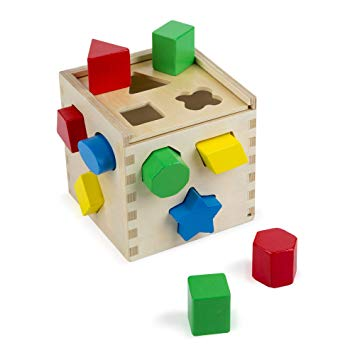
\includegraphics[scale=0.5]{toy.jpg}
    \end{figure}
    \end{frame}

\end{document}

